% !TeX root = main.tex
\documentclass[a4paper,10pt]{article}
\usepackage{refs/trymtex}
\usepackage{csquotes}
\usepackage[backend=biber]{biblatex}
\usetikzlibrary{matrix}
\usetikzlibrary{positioning,arrows,shapes,calc}

\addbibresource{refs/references.bib}

\title{Numerical Solution of Differential Equations - Project 1}
\author[1]{Sæther, Trym}
\author[1]{Haugen, Tor Ludvig Løvold}
\affil[1]{Department of Mathematical Sciences, NTNU}
\date{\today}

\begin{document}

\maketitle

\newpage
\begin{abstract}
    We develop and analyze a reaction-diffusion SIR model on a 2D domain, coupling an explicit reaction update with a Crank--Nicolson approach for diffusion. The method is unconditionally stable in the linearized case and second-order accurate when time and space steps scale appropriately. Numerical tests illustrate infection spread patterns under varied initial conditions and spatially/time-dependent infection rates, highlighting both the scheme’s stability and the simplifying assumptions that limit real-world applicability.
\end{abstract}
    
\tableofcontents
\newpage

\chapter{Introduction}
\section{Theory}

\subsection{Overview of the Numerical Method}

We consider the reaction-diffusion equation
\[
  u_t \;=\; \mu\,u_{xx} \;+\; f(u),
  \quad x \in (0,L),\quad t>0,
\]
where \(\mu > 0\) is the diffusion coefficient and \(f(u)\) is a reaction term. We discretize
space by dividing \((0,L)\) into \(M+1\) subintervals of uniform width \(h = L/(M+1)\), so
the grid points are \(x_m = m\,h\) for \(m = 0,\dots,M+1\). In time, we use a step \(k>0\),
so \(t_n = n\,k\). Let \(U_m^n \approx u(x_m,t_n)\). Then we define the dimensionless
parameter
\[
  r \;=\; \frac{\mu\,k}{h^2}.
\]
The scheme combines a Crank–Nicolson-like step for the diffusion term with an explicit
component for the reaction. it approximates the spatial derivative at the midpoint between time steps.
It is unconditionally stable and second-order accurate in time and space. Concretely, each time-step consists of:

\begin{enumerate}
  \item \emph{Predictor}: approximate the diffusion term in a semi-implicit manner and
        add an explicit reaction increment:
        \[
          U_m^\star
          \;=\; U_m^n
          \;+\; \frac{r}{2}\bigl(\delta_x^2 U_m^\star + \delta_x^2 U_m^n\bigr)
          \;+\; k\,f\bigl(U_m^n\bigr), \quad \text{where} \quad \delta_x^2 U_m^n = U_{m+1}^n - 2\,U_m^n + U_{m-1}^n.
        \]


  \item \emph{Corrector}: apply a midpoint update for the reaction:
        \[
          U_m^{n+1}
          \;=\; U_m^\star
          \;+\; \tfrac{k}{2}\,\Bigl(f\bigl(U_m^\star\bigr) - f\bigl(U_m^n\bigr)\Bigr).
        \]
\end{enumerate}

Visually the scheme can be illustrated with a stencil as shown below. Clearly showing the discretization of
the domain and how this is used to calculate the next value in time with the diffusion term calculated
semi-implicitly and the reaction term explicity.


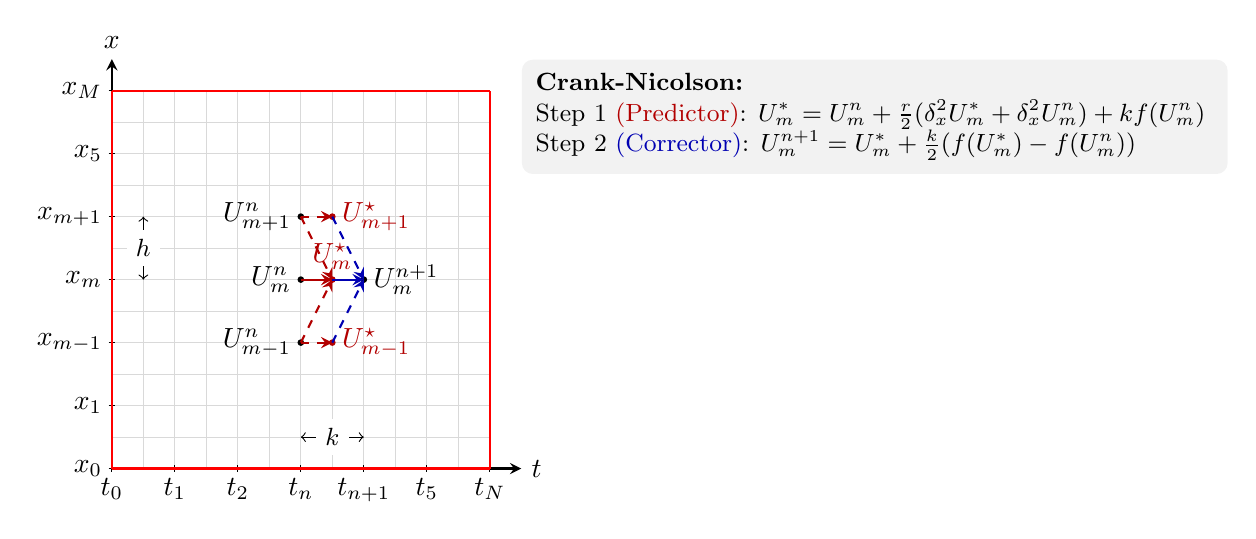
\begin{tikzpicture}[scale=0.8]
  % Define colors
  \colorlet{pointcolor}{black}
  \colorlet{gridcolor}{gray!30}
  \colorlet{predictorcolor}{red!70!black}
  \colorlet{correctorcolor}{blue!70!black}

  % Axes
  \draw[-stealth, thick] (0,0) -- (6.5,0) node[right] {$t$};
  \draw[-stealth, thick] (0,0) -- (0,6.5) node[above] {$x$};

  % Grid
  \draw[step=0.5cm, gridcolor, thin] (0,0) grid (6,6);

  % Add time labels
  \foreach \x/\label in {0/0, 1/1, 2/2, 3/n, 4/{n+1}, 5/5, 6/N} {
  \node[below] at (\x,0) {$t_{\label}$};
  \draw (\x,-0.05) -- (\x,0.05);
  }

  % Add space labels
  \foreach \y/\label in {0/0, 1/1, 2/{m-1}, 3/m, 4/{m+1}, 5/5, 6/M} {
  \node[left] at (0,\y) {$x_{\label}$};
  \draw (-0.05,\y) -- (0.05,\y);
  }

  % Highlight grid points for Crank-Nicolson stencil
  \fill[pointcolor] (3,3) circle (1.5pt) node[left] {$U_m^n$};
  \fill[pointcolor] (4,3) circle (1.5pt) node[right] {$U_m^{n+1}$};
  \fill[pointcolor] (3,2) circle (1.5pt) node[left] {$U_{m-1}^n$};
  \fill[pointcolor] (3,4) circle (1.5pt) node[left] {$U_{m+1}^n$};

  % Add intermediate points for the predictor step
  \fill[predictorcolor] (3.5,3) circle (1.5pt) node[above] {$U_m^\star$};
  \fill[predictorcolor] (3.5,2) circle (1.5pt) node[right] {$U_{m-1}^\star$};
  \fill[predictorcolor] (3.5,4) circle (1.5pt) node[right] {$U_{m+1}^\star$};

  % Show the predictor step with arrows
  \draw[->,-stealth, predictorcolor, thick] (3,3) -- (3.5,3);
  \draw[->,-stealth, predictorcolor, thick, dashed] (3,2) -- (3.5,3);
  \draw[->,-stealth, predictorcolor, thick, dashed] (3,4) -- (3.5,3);
  \draw[->,-stealth, predictorcolor, thick, dashed] (3,2) -- (3.5,2);
  \draw[->,-stealth, predictorcolor, thick, dashed] (3,4) -- (3.5,4);

  % Show the corrector step with arrows
  \draw[->,-stealth, correctorcolor, thick] (3.5,3) -- (4,3);
  \draw[->,-stealth, correctorcolor, thick, dashed] (3.5,2) -- (4,3);
  \draw[->,-stealth, correctorcolor, thick, dashed] (3.5,4) -- (4,3);

  % Step size annotations
  \draw[<->] (3,0.5) -- (4,0.5) node[midway, fill=white, font=\small] {$k$};
  \draw[<->] (0.5,3) -- (0.5,4) node[midway, fill=white, font=\small] {$h$};

  % Boundary and initial conditions
  \draw[red, thick] (0,0) -- (0,6);
  \draw[red, thick] (6,0) -- (6,6);
  \draw[red, thick] (0,0) -- (6,0);
  \draw[red, thick] (0,6) -- (6,6);

  % boundary labels MÅ FIKSES!

  % Crank-Nicolson scheme visualization
  \node[below right, align=left, font=\small, fill=gray!10, rounded corners, inner sep=5pt]
  at (6.5,6.5) {
  \textbf{Crank-Nicolson:}\\
  Step 1 \textcolor{predictorcolor}{(Predictor)}: $U_m^* = U_m^n + \frac{r}{2}(\delta_x^2 U_m^* + \delta_x^2 U_m^n) + k f(U_m^n)$ \hspace{5pt} \\
  Step 2 \textcolor{correctorcolor}{(Corrector)}: $U_m^{n+1} = U_m^* + \frac{k}{2}(f(U_m^*) - f(U_m^n))$
  };
\end{tikzpicture}

For the boundary conditions, either Dirichlet, Neumann, or Robin, one sets or solves for the boundary
values \(U_0^n\), \(U_{M+1}^n\) at each step as usual.

\subsection{Error Analysis}
To analyze the correctness of the scheme it is critical to determine both the consistency and stability of the
scheme. This is because a numerical method converges, as in, produces the true PDE solution as the grid is refined,
if and only if it is both consistent and stable. Consistency ensures the scheme’s discrete equations capture
the differential equation correctly. Stability ensures errors do not grow uncontrollably. Without both, one cannot
guarantee convergence.


\subsubsection{Consistency}
To determine the consistency of the modified Crank-Nicolson scheme for the PDE with the linear reaction term
$f(u) = au$, we analyze the local truncation error (LTE) by substituting the exact solution into our
numerical scheme.

\begin{theorem}{Local truncation error for the modified Crank-Nicolson}{lte_cn}
  For the PDE $u_t = \mu u_{xx} + au$ with constant $a$, the modified Crank-Nicolson scheme with steps $h$ (space)
  and $k$ (time) has local truncation error
  \[
    \|\tau_m^n\| = \mathcal{O}\!\left(k +\tfrac{h^4}{k}\right)
  \]
  where $u_m^n = u(x_m,t_n)$ is the exact solution and $U_m^n$ its numerical approximation.

  Under parabolic scaling $k \sim h^2$, the scheme achieves second-order accuracy:
  \[
    \|\tau_m^n\| = \mathcal{O}\!\left(h^2 + k^2\right)
  \]
\end{theorem}


\begin{proof}[Proof of Theorem~\ref{thm:lte_cn}]
  We analyze the truncation error by examining how the exact solution satisfies the numerical scheme.

  First, consider the central difference approximations for the second derivatives:
  \begin{align*}
    \delta_x^2 u_m^n     & = h^2u_{xx}(x_m,t_n) + \mathcal{O}(h^4)       \\
    \delta_x^2 u_m^\star & = h^2u_{xx}(x_m,t_n) + \mathcal{O}(h^4 + k^4)
  \end{align*}

  \textit{Step 1 (Predictor):} Substituting the exact solution into the first stage:
  \begin{equation}
    u_m^\star = u_m^n + \frac{r}{2}\left(\delta_x^2 u_m^\star + \delta_x^2 u_m^n\right) + kau_m^n = u_m^n + \frac{\mu k}{2}u_{xx}(x_m,t_n) + kau_m^n + \mathcal{O}(h^4 + k^4)
  \end{equation}
  \textit{Step 2 (Corrector):} For the second stage:
  \begin{align*}
    u_m^{n+1} & = u_m^\star + \frac{k}{2}(au_m^\star - au_m^n)
  \end{align*}

  From the PDE, we know $u_t = \mu u_{xx} + au$ and can derive expressions for higher time derivatives. Using Taylor expansion:
  \begin{align*}
    u(x_m,t_n+k) & = u_m^n + ku_t + \frac{k^2}{2}u_{tt} + \frac{k^3}{6}u_{ttt} + \mathcal{O}(k^4)
  \end{align*}

  Comparing this with our numerical solution, we obtain:
  \begin{align*}
    U_m^{n+1} - u_m^{n+1} & = \mathcal{O}(k^2 + h^4)
  \end{align*}

  The local truncation error per step is thus:
  \begin{align*}
    \|\tau_m^{n+1}\| & = \frac{|U_m^{n+1} - u_m^{n+1}|}{k} = \mathcal{O}\left(k + \frac{h^4}{k}\right)
  \end{align*}

  Under the parabolic scaling $k \sim h^2$, we have $\frac{h^4}{k} \sim h^2$, yielding second-order accuracy:
  \begin{align*}
    \|\tau_m^{n+1}\| = \mathcal{O}(h^2 + k^2)
  \end{align*}
\end{proof}

Hence, as stated in the theorem, if we choose \(k\) and \(h\) so that \(k \approx \mathrm{const}\times h^2\),
the method achieves second-order accuracy in both time and space.

\subsubsection{Stability Analysis}

We investigate whether the scheme can tolerate large time steps without amplification of numerical errors, thus
satisfing the conditions for stability.
For linear problems
\(\,u_t = \mu\,u_{xx} + a\,u,\) a von~Neumann analysis is done to see whether
this is true.

\begin{theorem}{von Neumann Stability for modified Crank--Nicolson}{von_neumann_cn}
  The modified Crank--Nicolson scheme for the PDE with a linear reaction term $f(u) = au$ is unconditionally
  stable for any choice of step sizes $h$ and $k$, as the amplification factor $\xi$ satisfies:
  \[
    |\xi| \leq 1 + Ck
  \]
  for some constant $C$ independent of step sizes.
\end{theorem}

\begin{proof}[Proof of Theorem~\ref{thm:von_neumann_cn}]
  We apply von Neumann stability analysis by studying how individual Fourier modes $U_m^n = \xi^n e^{i\beta mh}$
  evolve under our scheme, where $\beta$ is the wave number.

  As previously statet the PDE with a linear reaction term $f(u) = au$, the two-stage modified Crank--Nicolson
  scheme is given by:
  \begin{align*}
    U_m^\star & = U_m^n + \frac{r}{2}\left(U_{m+1}^\star - 2U_m^\star + U_{m-1}^\star + U_{m+1}^n - 2U_m^n + U_{m-1}^n\right) + kaU_m^n \\
    U_m^{n+1} & = U_m^\star + \frac{ka}{2}(U_m^\star - U_m^n)
  \end{align*}

  Substituting the Fourier mode $U_m^n = \xi^n e^{i\beta mh}$ and letting
  $U_m^\star = \xi^n \xi^\star e^{i\beta mh}$, we can use the identity
  $e^{i\beta (m+1)h} - 2e^{i\beta mh} + e^{i\beta (m-1)h} = -4\sin^2(\beta h/2)e^{i\beta mh}$ and derive:

  \begin{align*}
    \xi^\star & = \frac{1 - r\sin^2(\beta h/2) + ka}{1 + 2r\sin^2(\beta h/2)}
  \end{align*}

  For the second stage:
  \begin{align*}
    \xi^{n+1} & = \xi^n\left[\xi_\star\left(1 + \frac{ka}{2}\right) - \frac{ka}{2}\right]
  \end{align*}

  Therefore, the amplification factor is:
  \begin{align*}
    \xi & = \frac{\left(1 - r\sin^2(\beta h/2) + ka\right)\left(1 + \frac{ka}{2}\right) - \frac{ka}{2}\left(1 + 2r\sin^2(\beta h/2)\right)}{1 + 2r\sin^2(\beta h/2)}
  \end{align*}

  After algebraic simplification, and substituting $s = \sin^2(\beta h/2)$:
  \begin{align*}
    \xi & = \frac{1 - rs(1 + \tfrac{3}{2}ka) + ka + \tfrac{1}{2}k^2a^2}{1 + 2rs}
  \end{align*}

  Then for $a \geq 0$ and any $r > 0$, both numerator and denominator are positive with $\xi(s) < 1$ for all
  $s \in [0,1]$.

  \medskip

  For $a < 0$, the worst case occurs at $s = 0$, giving:
  \begin{align*}
    \xi(0) & = 1 + ka + \frac{k^2a^2}{2} = 1 + ka\left(1 + \frac{ka}{2}\right)
  \end{align*}

  For sufficiently small $k$:
  \begin{align*}
    |\xi(0)| & \leq 1 + |a|k(1 + |a|k/2)
  \end{align*}

  Therefore, $|\xi| \leq 1 + Ck$ with $C = |a|(1 + |a|k/2) \approx |a|$ for small $k$, confirming the scheme is unconditionally stable.
\end{proof}


\subsubsection{Global Error and Convergence}

\begin{theorem}{Lax Equivalence and Convergence of Crank--Nicolson}{cn_convergence}
  Since the modified Crank--Nicolson scheme is both consistent and stable, by the Lax Equivalence Theorem
  (Theorem~\ref{thm:lax}), it is convergent. Under the parabolic scaling $k \sim h^2$, the scheme achieves
  second-order convergence. Thus the global error satisfies:
  \[
    \|e_m^n\| = \mathcal{O}\!\left(h^2 + k^2\right)
  \]

\end{theorem}

Hence the proposed two-stage method inherits the main advantages of Crank--Nicolson (robust stability, second-order behavior) while treating the reaction term explicitly.

\subsection{Numerical Verification}
We verify the theoretical results by simulating the reaction-diffusion equation with a linear reaction term.
Here the reaction term is given by \(f(u) = au\) with \(a = 1\), and the diffusion coefficient is set to \(\mu = 1\).

\begin{figure}[H]
  \centering
  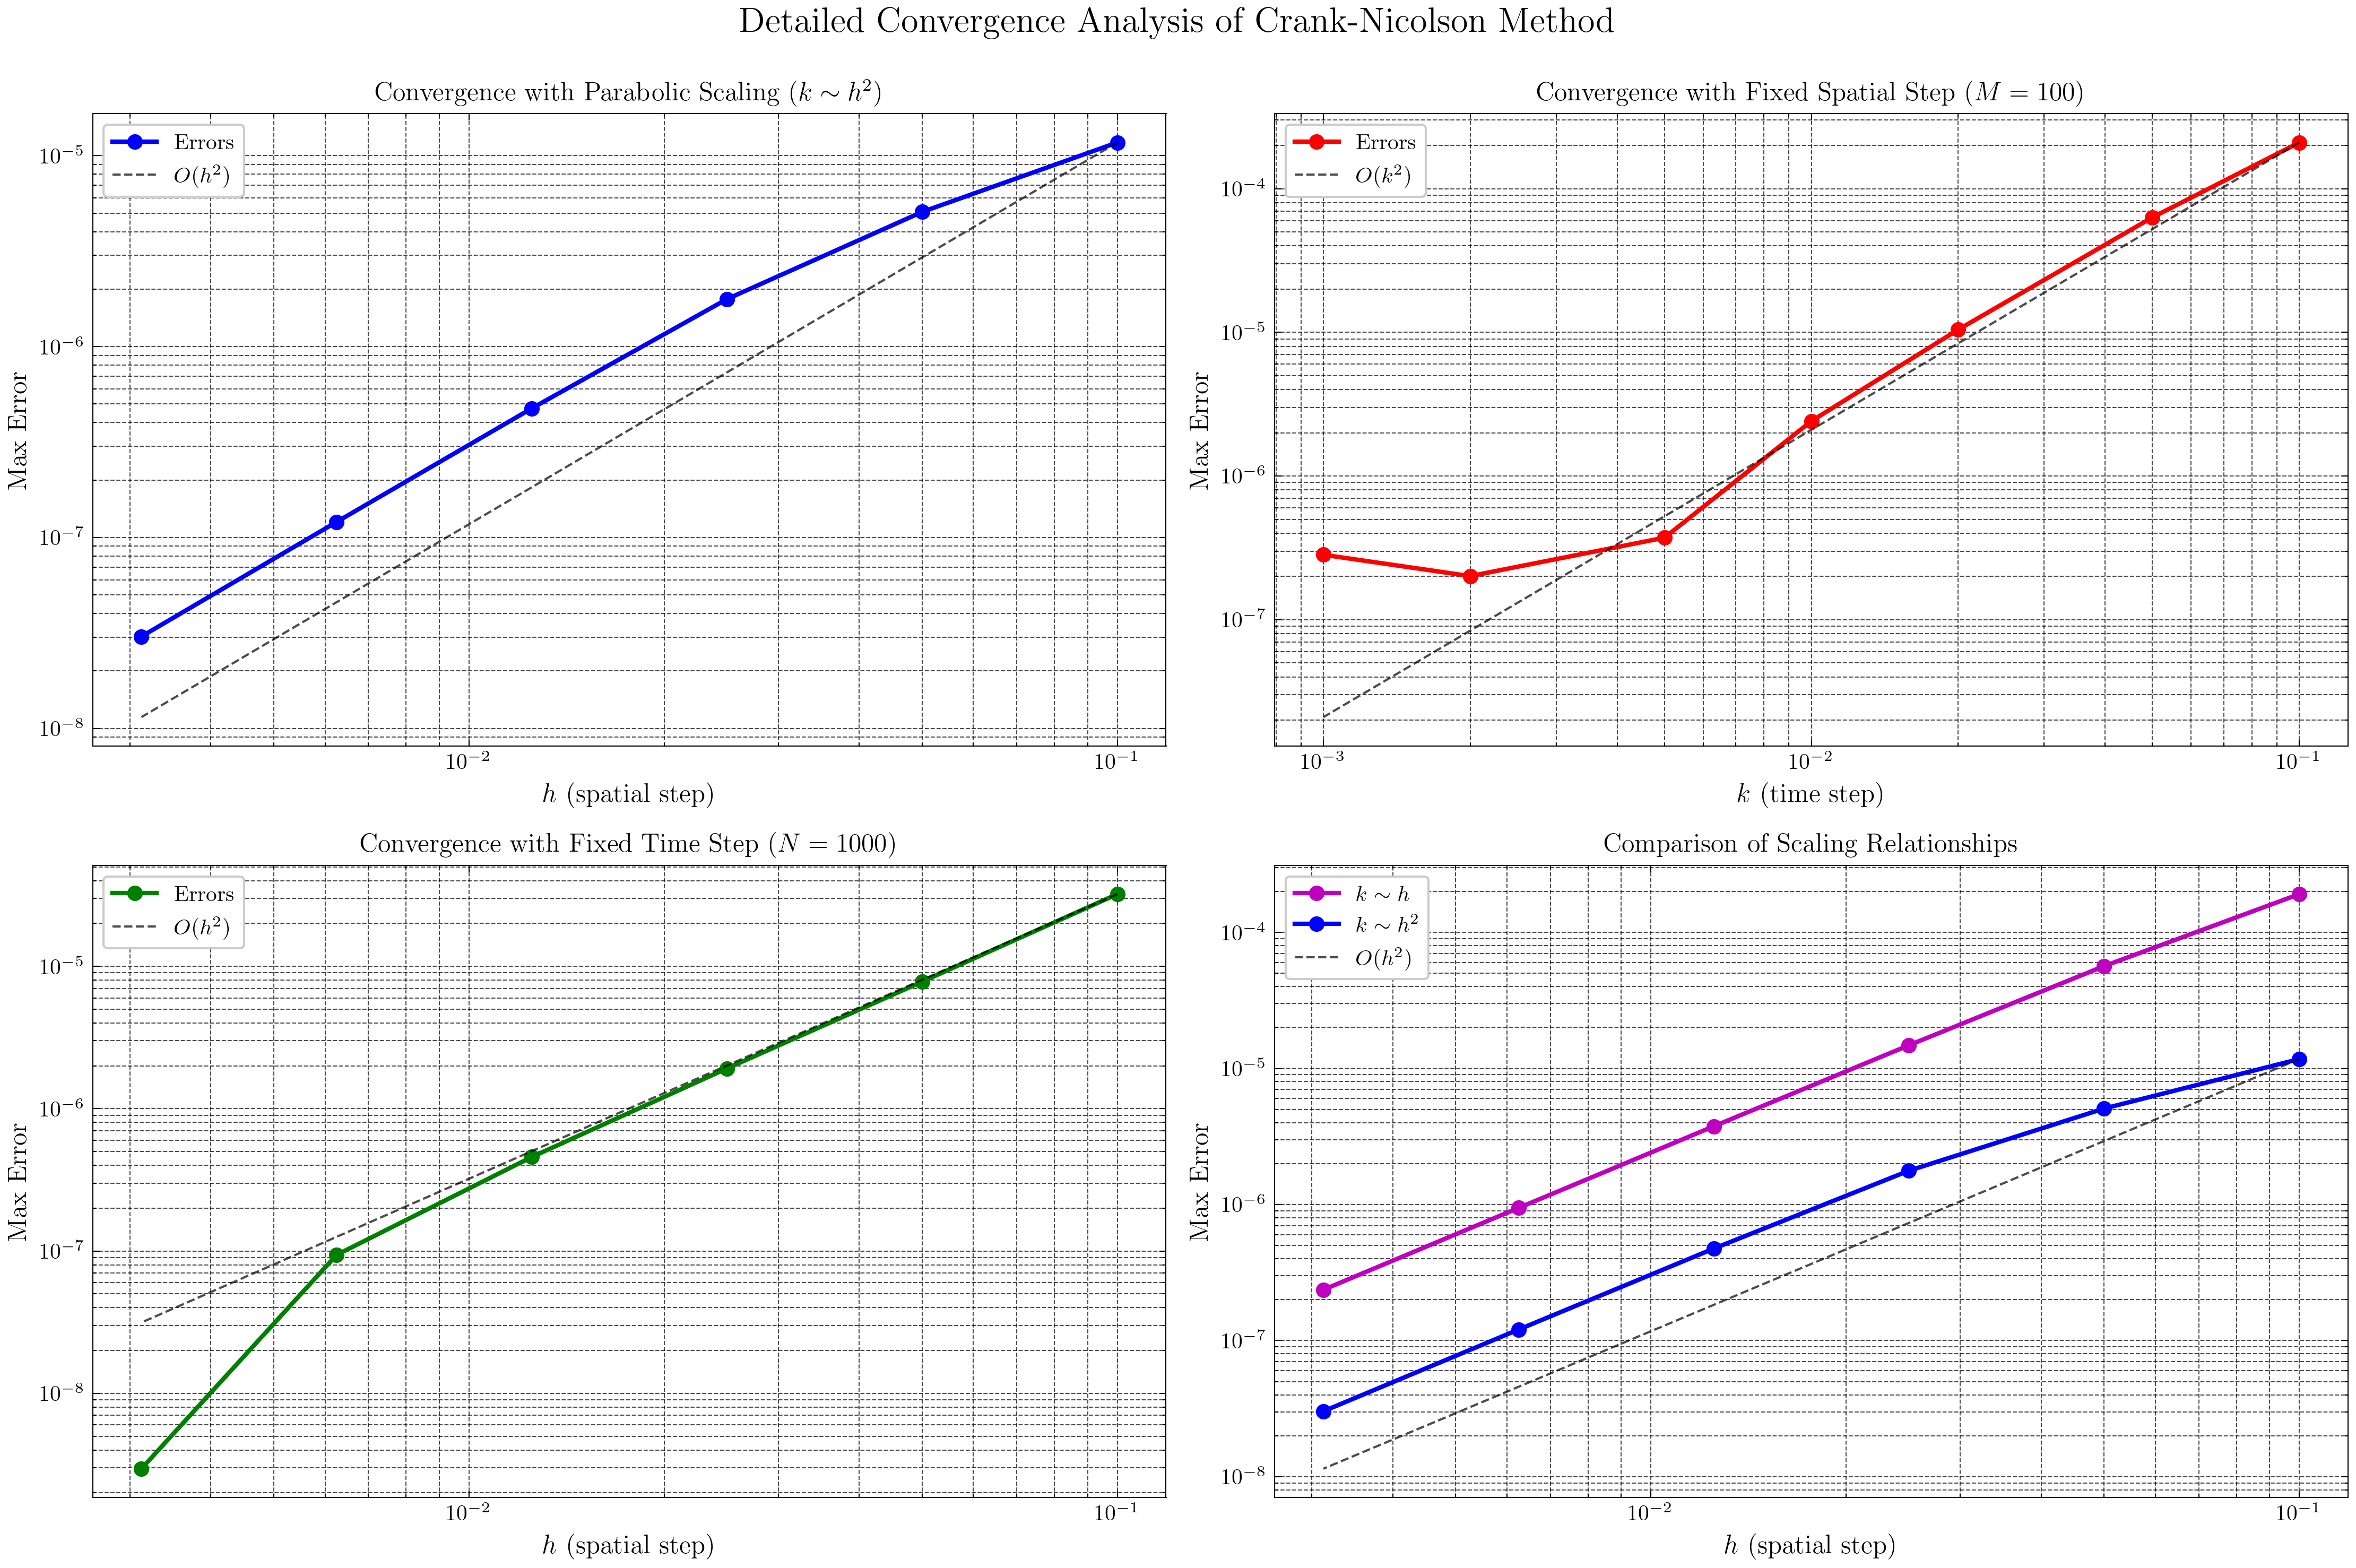
\includegraphics[width=0.5\textwidth]{figures/convergence_analysis_2d.png}
  \caption{Convergence analysis of the modified Crank--Nicolson scheme for the reaction-diffusion equation with a linear reaction term.}
  \label{fig:convergence_analysis_2d}
\end{figure}

The figure shows the convergence of the numerical solution to the exact solution as the grid is refined. The error decreases quadratically with respect to both \(h\) and \(k\), confirming the second-order accuracy of the scheme.

We can also confirm that choosing a parabolic scaling \(k \propto h^2\) yields second-order convergence.



\section{Application: Spatial-Temporal SIR Model}

We study the spatial-temporal spread of a disease by extending the classic SIR model to two spatial dimensions. 
This results in a reaction-diffusion system for \((S,I)\) on a square domain \(\Omega = [0,L]\times [0,L]\). As
discussed in the theory section this is a good candidate for the modified Crank--Nicolson scheme.

\subsection{Model Formulation and Modifications}

A classical SIR system tracks susceptible \(S\), infected \(I\), and removed \(R\). 
At a single location, one has
\[
  \begin{cases}
    S'(t) \;=\; -\beta\,S(t)\,I(t),\\[4pt]
    I'(t) \;=\; \beta\,S(t)\,I(t)\;-\;\gamma\,I(t),\\[4pt]
    R'(t) \;=\;\gamma\,I(t).
  \end{cases}
\]
Here \(\beta\) is the infection rate and \(\gamma\) the recovery rate. And \(S+I+R=1\) when normalized to a 
unit population.

To allow disease to spread across a region, we introduce diffusion of \(S\) and \(I\).
\[
  \begin{cases}
    S_t \;=\; -\beta\,S\,I \;+\;\mu_S\,\Delta S,\\[6pt]
    I_t \;=\; \beta\,S\,I \;-\;\gamma\,I \;+\;\mu_I\,\Delta I,
  \end{cases}
  \quad (x,y)\in\Omega,\;t>0.
\]
We set \(R=1-S-I\) and update it via \(R_t = \gamma\,I\). Here \(\Delta = \partial_x^2 + \partial_y^2\) is the 2D 
Laplacian, and \(\mu_S,\mu_I\) are diffusion coefficients.


Additionally to let this modell be better applicable to realistic scenarios we modify \(\beta\) to be dynamic in 
space and time, i.e.\ \(\beta = \beta(x,y,t)\). Physically, it might be higher in densely populated areas or 
vary over time for example periodic public gatherings.

\subsection{Numerical Implementation}

\subsubsection{Discretization of the Domain}

We subdivide \(\Omega=[0,L]\times [0,L]\) into an \(\!M\times M\) grid. Let \(h=L/M\) so that the grid points in
each direction are \(x_i = i\,h\), for \(i=0,\dots,M\). Combining,
\(\bigl\{(x_i, y_j)\bigr\}\) yields \(M^2\) internal variables for each unknown (\(S\) and \(I\)).

We approximate \(\Delta u\approx \partial_x^2u+\partial_y^2u\) by standard central differences. In one dimension 
(size \(M\)), the matrix for second differences is tridiagonal:
\[
  L_{\text{1D}} \;=\; \frac{1}{h^2}\,\begin{bmatrix}
    -2 & 1 &         &   &     \\
     1 & -2 & 1      &   &     \\
       & 1  & \ddots & \ddots &\\
       &    & \ddots & -2 & 1   \\
       &    &        & 1 & -2
  \end{bmatrix}.
\]
To handle a 2D Laplacian, we form \(L_{\text{2D}} = \text{kron}(I,L_{\text{1D}}) + \text{kron}(L_{\text{1D}},I)\), 
where \(\text{kron}\) is the Kronecker product and \(I\) is the \(M\times M\) identity. This yields an 
\((M^2)\times(M^2)\) sparse matrix. In the code, \(\mathrm{laplacian()}\) returns precisely this matrix.

\subsubsection{Chosen Boundary Conditions and Parameters}

We use a no-flux boundary condition, effectively, \(\mu \Delta u\) is discretized so that outward flux is zero 
at the domain edges. This is reflected by the modified diagonal entries for the topmost and bottommost rows 
in \(L_{\text{1D}}\). This is typical of a homogeneous Neumann implementation in central differences.


In the code, \(\beta=3\) and \(\gamma=1\) are chosen as baseline infection and recovery rates, matching simpler 
1D SIR examples.  We set \(\mu_S\) and \(\mu_I\) to small values so that susceptible and infected individuals do 
not diffuse too quickly.  The domain is \(L=1\), and we choose \(M=50\), 50 intervals in each dimension, and a 
small time-step \(\text{dt} = 0.001\).  The simulation runs up to \(T=10\) units of time.


For the initial conditions there are three modes of “infected” initialization:
\begin{itemize}
  \item \(\texttt{n=0}\): Dense local infection in corners, using a Gaussian peak near \(\tfrac{L}{4},\tfrac{L}{4}\) plus its mirror.
  \item \(\texttt{n=1}\): A linear front of infection occupying the leftmost 20\% of the domain.
  \item \(\texttt{n=2}\): Several random patches within the interior, mimicking local clusters.
\end{itemize}
We let \(S=1 - I\) initially (with \(R=0\)).  The choice of \( \approx 0.01\) sets how large the initial 
infection fraction is.

\subsubsection{Beta function}
As previously stated, the SIR model is modified when a dynamic beta, meaning that beta is a function dependent on 
both time and space. This is implemented via:
\[
  \beta(x,y,t) 
  \;=\; \beta_0 \times \bigl[1 + 0.5\,e^{-100\,((x-\tfrac{L}{2})^2 + (y-\tfrac{L}{2})^2)}\bigr]
  \times \bigl[1 + 0.1 \sin(t-2)\bigr]\quad (\text{for }2\le t \le 2+\pi),
\]
and equals the constant \(\beta_0\) otherwise.

\subsection{Implementation Details}

\paragraph{Sparse Matrix Storage.}
Since our 2D Laplacian is large \((M^2\times M^2)\) but banded, we store it in sparse format via 
\(\texttt{diags}\), \(\texttt{eye}\), and \(\texttt{kron}\). This greatly reduces memory usage and speeds up 
matrix operations.  Each time-step, we multiply this matrix by \(\mathrm{S}\) and \(\mathrm{I}\) to account for 
diffusion.

\paragraph{Time-Stepping.}
Given \(\Delta t=\text{dt}\),
\[
  S^{n+1} 
  \;=\;
  S^n + \Delta t\,\Bigl[\mu_S\,L_{\text{2D}}\,S^n - \beta(x,y,t_n)\,S^n\,I^n\Bigr],
  \quad
  I^{n+1}
  \;=\;
  I^n + \Delta t\Bigl[\mu_I\,L_{\text{2D}}\,I^n + \beta\,S^n\,I^n - \gamma\,I^n\Bigr].
\]
We also update 
\(
  R^{n+1} = R^n + \Delta t\,\bigl[\gamma\,I^n\bigr].
\)
If \(\beta\) is dynamic, we compute \(\beta(x,y,t)\) each step before forming the infection source term.

\subsection{Justification of Choices}

\begin{itemize}
  \item \textbf{Domain and Grid:} We use a unit square \((0,1)\times (0,1)\) with a \(50\times 50\) mesh for a compromise between resolution and runtime. A larger mesh would capture finer diffusion details but slow the simulation significantly.
  \item \textbf{Time Step:} We pick \(\Delta t = 0.001\) so that the PDE solution remains stable for the chosen parameters; in principle the method could allow larger \(\Delta t\), but high \(\beta\) and multiple infection clusters can demand refined time resolution for accurate capturing of fast infection waves.
  \item \textbf{Boundary Conditions:} A near--Neumann approach ensures people cannot exit or enter the domain, consistent with a self-contained population. 
  \item \textbf{Parameter Values:} Baseline \(\beta=3\) and \(\gamma=1\) produce a typical SIR behavior in well-known 1D test cases. Varying \(\mu_S\) and \(\mu_I\) influences how quickly each group moves about the domain.
  \item \textbf{Initial Infections:} We tested three distinct initial distributions (\texttt{n=0,1,2}) to see how infection geometry affects overall spread. The optional \(\texttt{dynamic\_beta}\) toggles a time- and space-dependent infection rate to model ephemeral gatherings or hotspots.
\end{itemize}

\subsection{Code Commentary}

\paragraph{Structure.}
The \(\texttt{SIRSimulation}\) class encapsulates domain setup, matrix assembly, initial conditions, and time-stepping (\(\texttt{step}\)). The 2D arrays \(S,I,R\) are flattened to vectors of length \(M^2\). 

\paragraph{Laplacian.}
The method \(\texttt{laplacian()}\) constructs the 1D second-difference operator as \(\texttt{L}\), then forms the 2D operator via Kronecker products. The diagonal near the boundary is adjusted so that the first and last rows have \(-1\) on the diagonal, consistent with no-flux or partial Neumann boundary approximations.

\paragraph{Integration Loop.}
At each step, we compute reaction terms \(\beta SI\) and \(\gamma I\), plus diffusion terms \(\mu_S L\cdot S\) and \(\mu_I L\cdot I\). We then do an explicit Euler update in time:
\[
  S \gets S + \mathrm{dt}\times(\text{diffusion} - \beta S I),\quad
  I \gets I + \mathrm{dt}\times(\text{diffusion} + \beta S I - \gamma I).
\]
An optional \(\beta\)-function can incorporate both a radial shape factor and a time-sinusoid, giving “hotspots” in space and fluctuating infection rates in time.

\paragraph{Animation.}
The \(\texttt{animate()}\) method updates in increments of 50 small steps (to keep the display from flickering). Matplotlib’s \(\texttt{FuncAnimation}\) drives the update loop, plotting the infected fraction in a 3D surface.

\subsection{Concluding Remarks on the SIR Simulation}

By combining a two-dimensional diffusion operator (for $S$ and $I$) with the usual SIR reaction terms, we capture how local infection spreads spatially. Our chosen domain and parameters illustrate various infection patterns:
\begin{itemize}
  \item \textbf{Small \(\mu_S,\mu_I\)}: keeps population mostly localized, leading to distinct infection clusters.
  \item \textbf{Modified \(\beta(x,y,t)\)}: represents spatiotemporal heterogeneity, e.g.\ higher infection rates in the central region or for certain times.
\end{itemize}
Though we used straightforward explicit Euler in time, the moderate diffusion and relatively small \(\Delta t\) suffice to maintain stability. More advanced time-stepping schemes (like Crank--Nicolson) could also be adapted for faster runs if necessary. Overall, our setup provides a flexible environment to explore how disease waves propagate and to visualize key features of spatio-temporal epidemics.

\section{Experiments and Results}

We simulate a two-dimensional SIR model with diffusion on a square domain \(\Omega = [0,L]\times [0,L]\) using a \(50\times 50\) grid.
The diffusion coefficients are set to \(\mu_S = 0.001\) and \(\mu_I = 0.001\), while the infection rate \(\beta=3.0\) is modified to be spatially and temporally dependent, as described in the previous section.

The initial conditions are chosen at random, with random positions for the infected individuals, and the simulation runs for \(T=15\).
In this case, we have an event at \(t=8\) that increases the infection rate in the top half of the domain within a certain radius.

\begin{figure}[H]
  \centering
  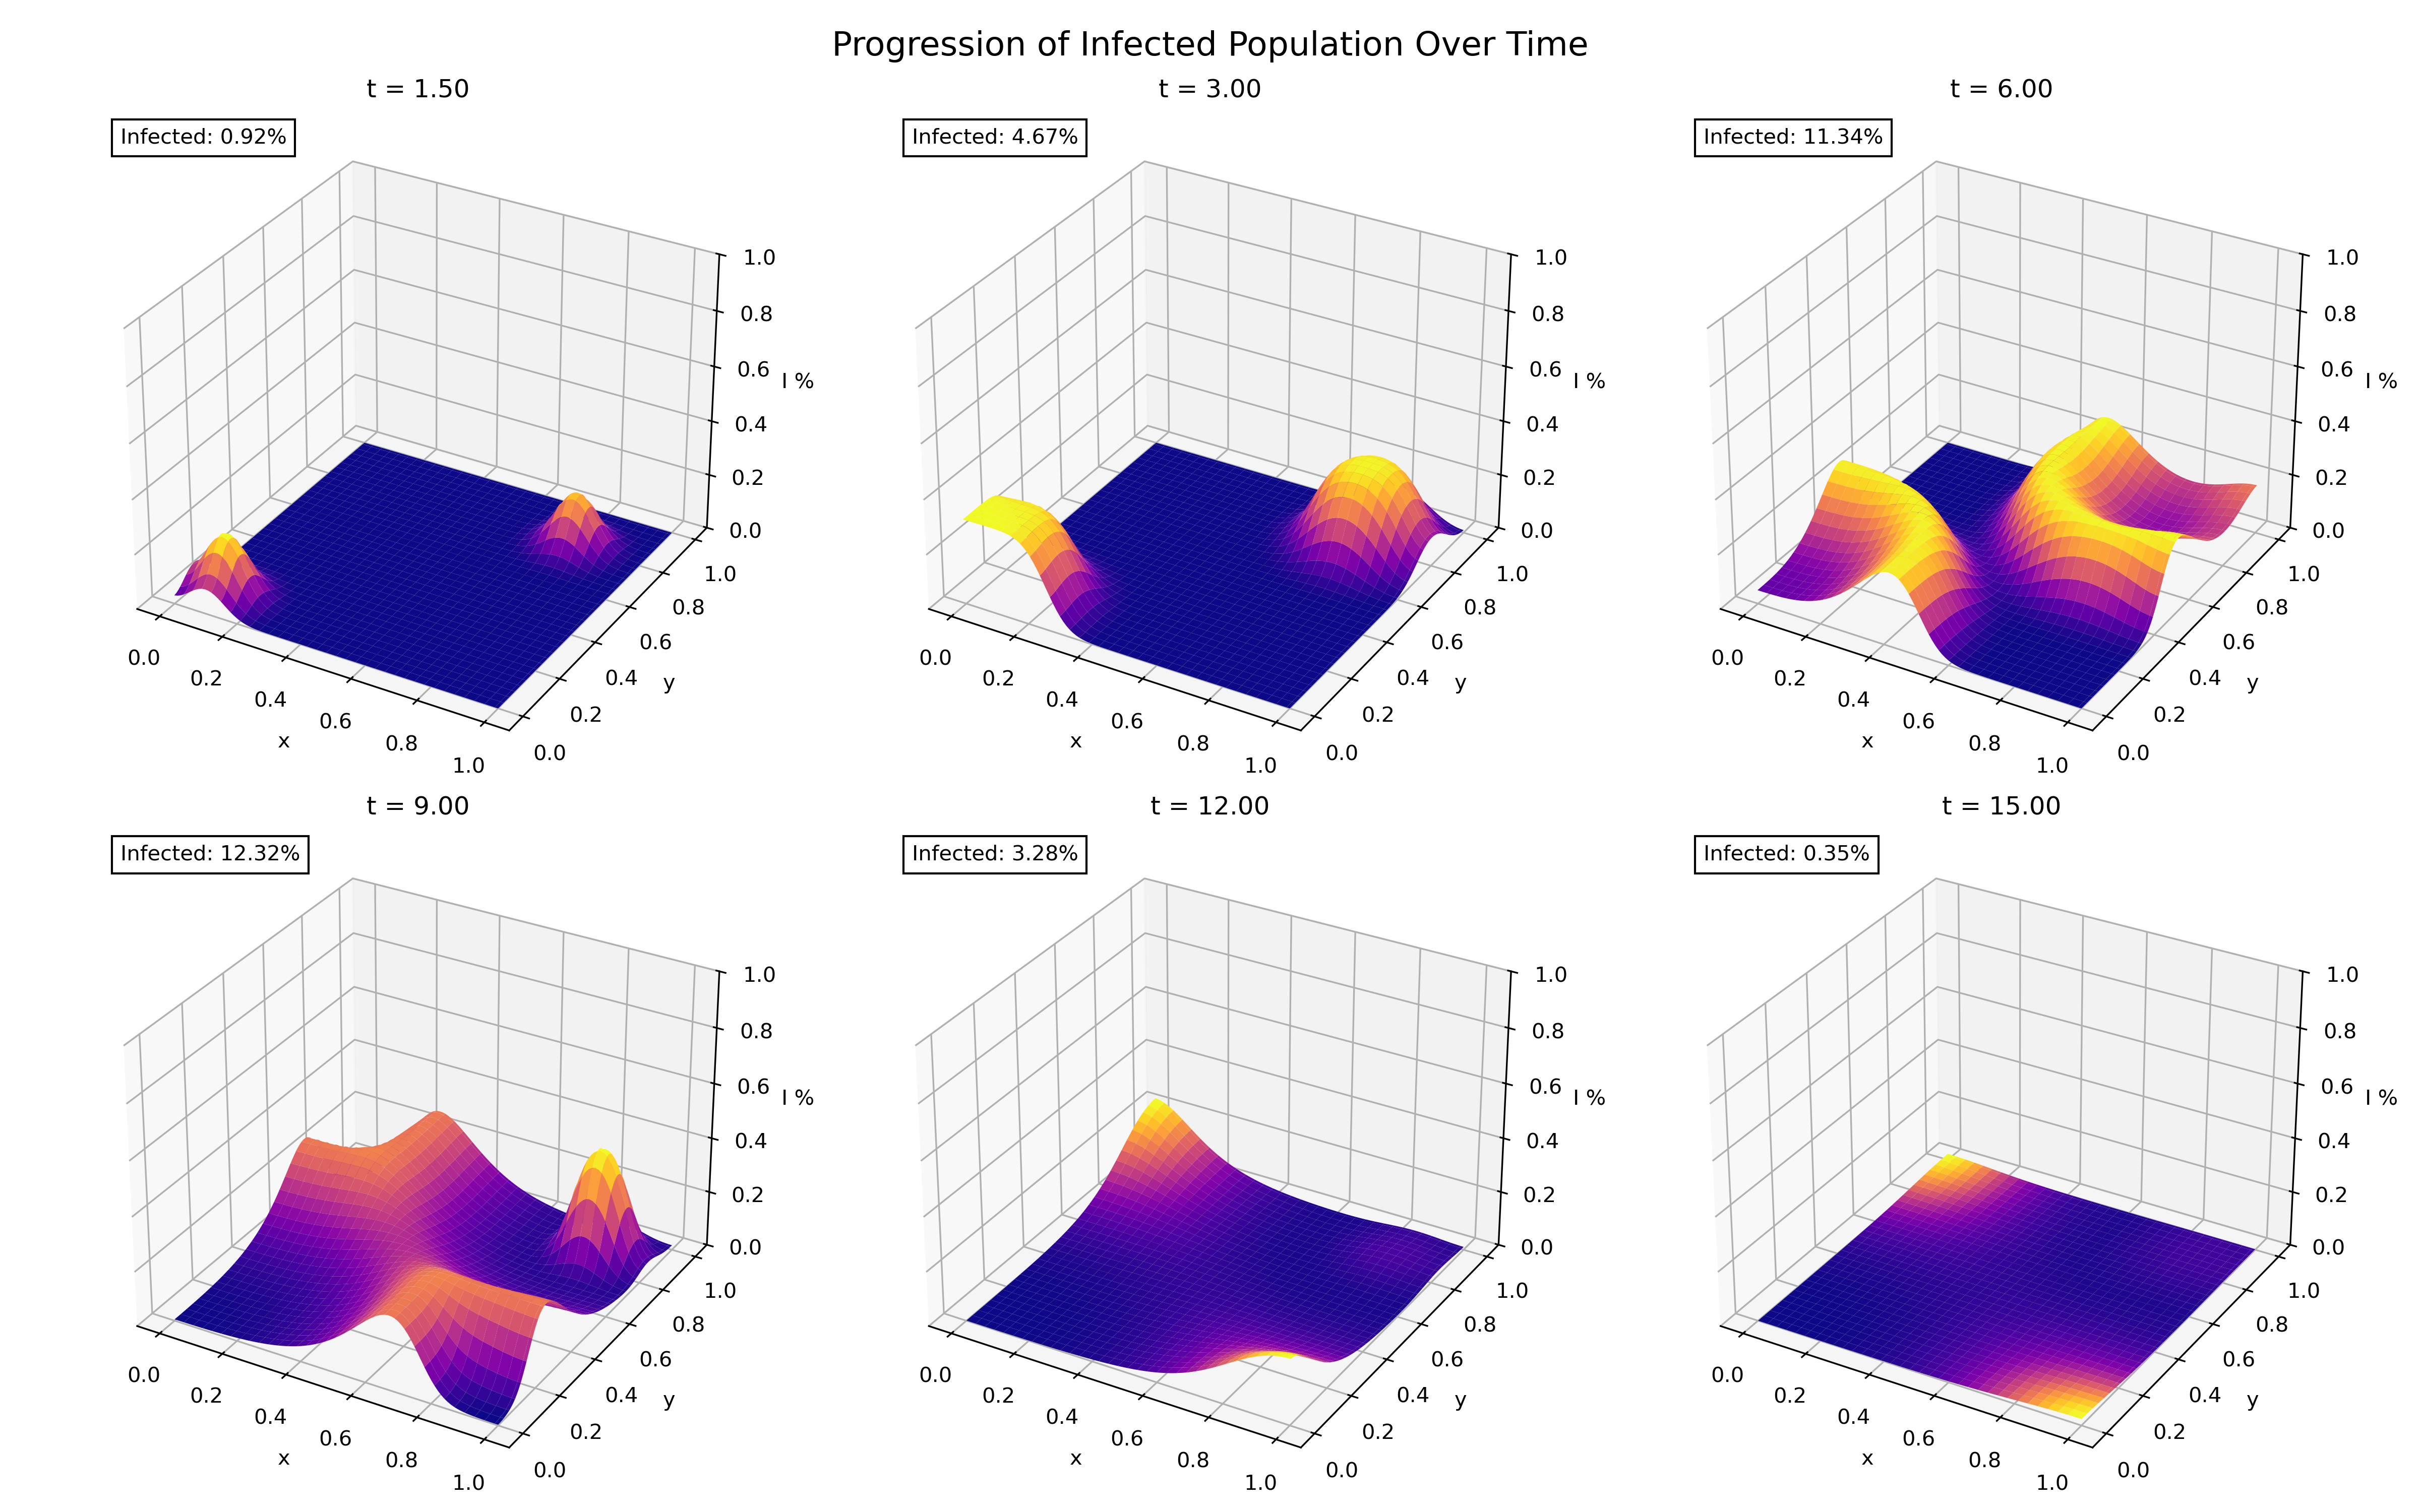
\includegraphics[width=0.9\textwidth]{figures/infected_progression.png}
  \caption{Infected population over time.}
  \label{fig:infected_progression}
\end{figure}

By combining a two-dimensional diffusion operator (for $S$ and $I$) with the usual SIR reaction terms, we capture how local infection spreads spatially. Our chosen domain and parameters illustrate various infection patterns:
\begin{itemize}
  \item \textbf{Small \(\mu_S,\mu_I\)}: keeps population mostly localized, leading to distinct infection clusters.
  \item \textbf{Modified \(\beta(x,y,t)\)}: represents spatiotemporal heterogeneity, e.g.\ higher infection rates in the central region or for certain times.
\end{itemize}
Though we used straightforward explicit Euler in time, the moderate diffusion and relatively small \(\Delta t\) suffice to maintain stability. More advanced time-stepping schemes (like Crank--Nicolson) could also be adapted for faster runs if necessary. Overall, our setup provides a flexible environment to explore how disease waves propagate and to visualize key features of spatio-temporal epidemics.


\section{Discussion}

\subsection{Theory versus Numerical Results}
In principle, the linear stability analysis applies most directly if \(f(u)\) is linear. Our tests used a strongly 
nonlinear infection term \(\beta\,S\,I\), so the unconditional stability partially hinges on the moderate size of 
\(\beta\) and small time steps in practice. The local truncation argument still informs us that spatial errors 
scale like \(h^2\) and temporal errors like \(k^2\). Numerically, we see outcomes 
consistent with that prediction, but if one pushed the ratio \(k/h^2\) too high or introduced extremely large 
\(\beta\), the scheme could exhibit instability or large phase errors. Thus, while the theoretical 
\(\mathcal{O}(h^2)\) accuracy remains a useful guideline, the real PDE problem is more delicate than a purely 
linear analysis suggests.

\subsection{Limitations of Numerical Scheme}
Although our numerical scheme is supported by a consistency and stability analysis for linearized 
problems, it faces some caveats. First, the reaction-diffusion equation with a fully nonlinear 
reaction \(f(u)\) may require additional care, especially if the reaction term grows quickly or exhibits stiff 
behavior. In that case, even though the scheme remains conditionally consistent, larger time steps may trigger 
inaccuracies in the reaction component.

\subsection{Limitations of SIR Model}
On the modeling side, our SIR setup simplifies many real-world complexities. The population is mostly uniformly 
distributed except for the small adjustments in \(\beta(x,y,t)\), travel into/out of the region is ignored, 
and we do not address other realistic processes. While these simplifications permit tractable PDE computations, 
it means our conclusions about how infection waves propagate may not translate directly to real world situations
\section{Conclusion}

\newpage
\section{Problem Description}

In this project, we will study reaction-diffusion equations. Such equations are given by
\begin{equation}
  u_t = \mu u_{xx} + f(u),
\end{equation}

where $\mu$ is some positive constant.
We will assume the reaction term $f(u)$ to be nonstiff, in the sense that explicit methods can be used to solve the ODE $u_t = f(u)$. As is well known, time-dependent PDEs with diffusion terms should be solved by implicit methods. Using implicit methods for solving the whole system requires solutions of nonlinear equations for each step, and we would all be happy to avoid that. One option would be to use an implicit method for the diffusion term and an explicit for the reaction.

We will use constant step sizes $h$ in the $x$-direction, and $k$ in the $t$-direction, so that $x_{m+1} = x_m + h$ and $t_{n+1} = t_n + k$. A scheme based on forward and backward Euler, together with a central difference in space could be
\begin{equation}
  \frac{1}{k} \nabla_t U_m^{n+1}  = \frac{\mu}{h^2} \delta_x^2 U_m^{n+1} + f(U_m^n)
\end{equation}
Which written out could be:
\begin{equation}
  U_m^{n+1}  = U_m^n + r \left( U_{m+1}^{n+1} - 2 U_m^{n+1} + U_{m-1}^{n+1} \right) + k f(U_m^n), \quad r = \frac{\mu k}{h^2}
\end{equation}

We now propose the following modification of the Crank-Nicolson scheme:
\begin{align*}
  U_m^*     & = U_m^n + r \left( \frac{1}{2} \delta_x^2 U_m^* + \frac{1}{2} \delta_x^2 U_m^n \right) + k f(U_m^n) \\
  U_m^{n+1} & = U_m^* + \frac{k}{2} \left( f(U_m^*) - f(U_m^n) \right).
\end{align*}

For pure diffusion ($f = 0$), this is nothing but the usual Crank-Nicolson scheme, and for a pure reaction equation ($\mu = 0$), it is nothing but a second-order explicit Runge-Kutta method.

\begin{railingbox}{Theory problem}
  Do a consistency/stability analysis of the proposed method (1) on a linear PDE, that is, let \(f(u) = au\) for some constant \(a\).
  For the stability analysis, you can choose whether you do a complete matrix analysis for the PDE on a given domain (e.g. \(x \in (0, 1)\)) with boundary conditions, or a Neumann analysis. Is the method unconditionally stable? What can be said about the global error?
  Formulate your results as a mathematical statements (lemmas or theorems) with proofs.
  Justify your theoretical results by numerical experiments.
\end{railingbox}


\begin{railingbox}{Application problem}
  In this exercise, we will look at a model from epidemiology; how an infectious disease will develop in space and time.
  At a given time \(t\), a population \(N\) can be divided into
  \begin{itemize}
    \item Susceptible \(S\): A person is susceptible if she/he may get the disease.
    \item Infective and infectious \(I\): A person is infective if she/he has the disease and is able to transfer it to others.
    \item Removed: \(R\) Part of the population that for some reason will never again be infected or infect others (immune, isolated from the population or dead).
  \end{itemize}
  The following model (SIR) is described in \cite{murray2002mathematical}, chapter 3, and describe the development of a disease over time:
  \begin{align}
    \frac{dS}{dt} & = -\beta SI, \quad \frac{dI}{dt} = \beta SI - \gamma I, \quad \frac{dR}{dt} = \gamma I  \label{eq:sir_model}
  \end{align}
  Notice that \(N(t) = S(t) + I(t) + R(t)\) is constant.
  In the following, we will assume a scaled model, so \(S\), \(I\) and \(R\) are the fraction of the population that are susceptible, infected and removed respectively. In this case, \(S(t) + I(t) + R(t) = 1\).
  The usual SIR model only describe how a disease may develop over time at one specific location, not how a disease is spread in space. Murray \cite{murray2002mathematical}, chapter 13, proposes the following modification to include spatial spread:
  \begin{align}
    S_t & = -\beta IS + \mu S \Delta S, \nonumber                            \\
    I_t & = \beta IS - \gamma I + \mu I \Delta I, \label{eq:sir_model_space}
  \end{align}
  where \(\Delta u = u_{xx} + u_{yy}\) (see the appendix). Your exercise is now: Try to understand the
  model. Choose an appropriate numerical scheme for solving the PDEs, and use this to study the spread of a disease. That is, at \(t = 0\) assume a small portion of the population is infected at some particular place, and see how the disease
  will spread from there. You are free to choose the domain, the parameters and boundary conditions, but you should be able to get some interesting results out of it. And you should justify your choices.
  As soon as you have a working model, play with it! As an example: In the present model, we assume that the population is equally distributed over the domain. You can for instance model a more dense populated area (or an event that gather a lot of people) by making \(\beta\) larger over there (and then dependent on \(x\)).
  Some hints:
  \begin{itemize}
    \item To get a certain feeling for the dynamics of the model, solve \eqref{eq:sir_model} first. As a first try, you can use \(\beta = 3\) and \(\gamma = 1\), but then change the parameters and see what happens. Use a standard ODE solver if you prefer.
    \item The diffusion parameters \(\mu^*\) describes how fast people are moving around. If your domain is small, you should probably use quite small diffusion parameters.
    \item For a full score, the 2d problem should be solved. But if this seems difficult, solve the 1d problem first.
  \end{itemize}
\end{railingbox}





\printbibliography

\appendix
\subsection{Appendix: Python Code}
\inputminted{python}{simulation/theory.py}
\inputminted{python}{simulation/SIRSimulation.py}


\end{document}
